\chapter{Ondas sonoras em fluidos}\label{ch:b2:sound-waves}

Conte os segundos entre o clarão e o trovão e divida por
três: essa é a distância em quilômetros. O som atravessa o ar a um
terço de quilômetro por segundo, a água a um quilômetro e meio, e
um aparelho de ultrassom cronometra os ecos de dentro do corpo com precisão de um
milionésimo de segundo para desenhar sua imagem. Este capítulo aplica a
mecânica dos fluidos dos \cref{ch:b2:euler-bernoulli,ch:b2:fluid-kinematics}
a um fluido em repouso perturbado por uma pequena ondulação de pressão, e reencontra a
\omterm{thm:b2:waves-on-strings:equation}{equação de d'Alembert}: a \omterm{thm:b2:sound-waves:equation}{velocidade do som}, o que carrega a
energia, o que quer dizer alto, como o som se espalha no espaço e por que uma sirene
muda de altura ao passar.

\section{A aproximação acústica}

\begin{definition}[Perturbação acústica]\label{def:b2:sound-waves:approximation}
\index{aproximação acústica}\index{sobrepressão}
Um fluido em repouso, de pressão uniforme $P_0$ e massa específica $\rho_0$, é
perturbado: $P = P_0 + p(M, t)$, $\rho = \rho_0 + \rho_1(M, t)$, velocidade
$\vect v(M, t)$. A \emph{aproximação acústica} guarda apenas a primeira
ordem nas pequenas grandezas $p$ (a \emph{sobrepressão}, ou pressão
acústica), $\rho_1$ e $\vect v$: $|p| \ll P_0$, $|\rho_1| \ll \rho_0$, $v \ll c$,
e a transformação sofrida por cada \omterm{def:b2:fluid-kinematics:particle}{partícula de fluido} é tão rápida
que ela não troca calor: é \emph{isentrópica}, com a
compressibilidade $\chi_S = \frac1\rho\bigl(\frac{\partial\rho}{\partial P}\bigr)_S$.
A gravidade é desprezada.
\end{definition}

\begin{theorem}[Ondas sonoras]\label{thm:b2:sound-waves:equation}
\index{velocidade do som}\index{equação de onda (acústica)}
Em primeira ordem, a \omterm{thm:b2:euler-bernoulli:euler}{equação de Euler}, a conservação da massa e a lei
isentrópica dizem
\[
\rho_0\frac{\partial\vect v}{\partial t} = -\operatorname{\vect{grad}}p , \qquad
\frac{\partial\rho_1}{\partial t} + \rho_0\operatorname{div}\vect v = 0 , \qquad
\rho_1 = \rho_0\chi_Sp ,
\]
e juntas elas dão a \omterm{thm:b2:waves-on-strings:equation}{equação de onda} para a \omterm{def:b2:sound-waves:approximation}{sobrepressão},
\[
\Delta p = \frac1{c^2}\frac{\partial^2p}{\partial t^2} , \qquad
c = \frac1{\sqrt{\rho_0\chi_S}} ,
\]
(a mesma para $\rho_1$ e para $\vect v$). Para um gás perfeito, $\chi_S =
1/\gamma P_0$ e
\[
c = \sqrt{\frac{\gamma P_0}{\rho_0}} = \sqrt{\frac{\gamma RT}{M}} :
\]
\qty{343}{m/s} no ar a \qty{20}{\degreeCelsius}, subindo \qty{0.6}{m/s}
por kelvin; \qty{1000}{m/s} no hélio; \qty{1480}{m/s} na água ($\chi_S =
\qty{4.5e-10}{Pa^{-1}}$).
\end{theorem}

\begin{proof}
Euler: o termo convectivo $\rho(\vect v\cdot\operatorname{\vect{grad}})\vect v$
é de segunda ordem, $\rho\,\partial_t\vect v \approx \rho_0\,\partial_t\vect v$, e
$\operatorname{\vect{grad}}P = \operatorname{\vect{grad}}p$. Massa: $\partial_t\rho +
\operatorname{div}(\rho\vect v) \approx \partial_t\rho_1 + \rho_0\operatorname{div}\vect v$.
Lei isentrópica: $\dd\rho = \rho\chi_S\,\dd P$ em primeira ordem. Tome o
divergente da primeira equação e a derivada temporal da segunda:
$\rho_0\partial_t\operatorname{div}\vect v = -\Delta p = -\partial_t^2\rho_1 = -\rho_0\chi_S
\partial_t^2p$. Para o gás perfeito, $PV^\gamma$ constante ao longo de uma transformação
isentrópica dá $\dd\rho/\rho = \dd P/\gamma P$, donde $\chi_S = 1/\gamma P$,
e $P_0/\rho_0 = RT/M$.
\end{proof}

\begin{remark}[Por que isentrópica]\label{rem:b2:sound-waves:laplace}
Newton calculou a \omterm{thm:b2:sound-waves:equation}{velocidade do som} com a compressibilidade isotérmica,
$\sqrt{P_0/\rho_0} = \qty{290}{m/s}$, $15\%$ baixa demais; Laplace percebeu que as
compressões são rápidas demais para que o calor flua entre as cristas quentes e
os vales frios --- ao longo de um período o calor difunde alguns micrômetros
(\cref{ch:b2:heat-conduction}), nada em comparação com um comprimento de onda ---
de modo que a transformação é adiabática e reversível, e $\gamma$ aparece.
A \omterm{thm:b2:sound-waves:equation}{velocidade do som} é assim uma medida direta de $\gamma$: $1.40$ para o
ar, $1.67$ para o argônio.
\end{remark}

\begin{omfigure}
\begin{tikzpicture}[font=\small, x=1cm, y=1cm, >=Stealth]
  \begin{scope}
    \draw[thick] (-3.2,-0.8) rectangle (3.2,0.8);
    \fill[omDef!25] (-0.6,-0.8) rectangle (0.6,0.8);
    \fill[omDef!8] (-0.35,-0.8) rectangle (0.95,0.8);
    \draw[omDef, dashed] (-0.35,-0.8) -- (-0.35,0.8) (0.95,-0.8) -- (0.95,0.8);
    \draw[omThm, very thick, ->] (-1.6,0) -- (-0.65,0) node[above, font=\footnotesize, pos=0.3] {$P(x)S$};
    \draw[omThm, very thick, ->] (1.6,0) -- (0.65,0) node[above, font=\footnotesize, pos=0.3] {$P(x+\dd x)S$};
    \node[font=\footnotesize] at (-0.6,-1.1) {$x$}; \node[font=\footnotesize] at (0.65,-1.1) {$x + \dd x$};
    \draw[omDef, ->] (-0.6,1.05) -- (-0.35,1.05) node[above, font=\footnotesize, pos=1.4] {$\xi(x)$};
    \node[font=\footnotesize] at (0,-1.7) {$\rho_0\,\partial_t v = -\partial_x p$, \quad $\rho_1 = -\rho_0\,\partial_x\xi = \rho_0\chi_S\,p$};
  \end{scope}
  \begin{scope}[xshift=8.2cm]
    \foreach \x in {-2.6,-2.45,...,2.6} {
      \pgfmathsetmacro{\d}{0.18*sin(deg(2.4*\x))}
      \draw[omDef, thick] ({\x+\d},-0.8) -- ({\x+\d},0.8);
    }
    \node[font=\scriptsize] at (-1.6,-1.1) {compressão}; \node[font=\scriptsize] at (0,-1.1) {rarefação}; \node[font=\scriptsize] at (1.6,-1.1) {compressão};
    \draw[omThm, thick, ->] (-0.4,1.1) -- (0.8,1.1) node[right, font=\footnotesize] {$c$};
    \node[font=\footnotesize] at (0,-1.7) {uma onda sonora plana: as fatias de fluido se juntam e se afastam};
  \end{scope}
\end{tikzpicture}

{\small À esquerda: uma fatia de fluido deslocada de $\xi(x, t)$ e empurrada pelas
pressões em suas faces; sua compressão fixa a \omterm{def:b2:sound-waves:approximation}{sobrepressão}.
À direita: uma onda sonora plana --- zonas alternadas de compressão e
rarefação que se movem a $c$, com o próprio fluido oscilando para a frente e para trás
segundo a direção de propagação (uma \omterm{prop:b2:waves-on-strings:chain}{onda longitudinal}).}
\end{omfigure}

\section{Ondas planas, impedância, intensidade}

\begin{proposition}[Onda sonora plana progressiva]\label{prop:b2:sound-waves:plane}
\index{impedância acústica}\index{intensidade acústica}\index{densidade de energia (acústica)}
Para uma onda plana $p = f(x - ct)$ que viaja rumo a $+x$, a velocidade do
fluido é segundo $x$, em fase com a \omterm{def:b2:sound-waves:approximation}{sobrepressão}, e
\[
p = Z\,v , \qquad Z = \rho_0c = \sqrt{\rho_0/\chi_S} ,
\]
onde $Z$ é a \emph{\omterm{prop:b2:sound-waves:plane}{impedância acústica}} do meio
(\unit{kg.m^{-2}.s^{-1}}): \qty{410}{kg.m^{-2}.s^{-1}} para o ar, \qty{1.5e6}{kg.m^{-2}.s^{-1}}
para a água, $\sim\qty{1.6e6}{kg.m^{-2}.s^{-1}}$ para o tecido mole,
\qty{4e7}{kg.m^{-2}.s^{-1}} para o aço. A onda transporta a densidade de energia e
a intensidade (potência por unidade de área, rumo a $+x$)
\[
e = \tfrac12\rho_0v^2 + \tfrac12\chi_Sp^2 , \qquad I = p\,v ,
\]
que obedecem a $\partial_te + \partial_xI = 0$; para a onda progressiva as duas
metades de $e$ são iguais e $I = p^2/Z = Zv^2$. Uma onda senoidal de
amplitude de pressão $p_m$ tem intensidade média $\langle I\rangle = p_m^2/2Z$.
\end{proposition}

\begin{proof}
Para $p = f(x - ct)$, $\rho_0\partial_tv = -\partial_xp = f'/c\cdot c\dots$: mais precisamente,
$\rho_0\partial_tv = -f'(x - ct)$, e $v = f(x - ct)/\rho_0c$ a satisfaz. O
termo potencial de $e$ é o trabalho armazenado ao comprimir o fluido
(uma compressão isentrópica de volume unitário por $\dd V/V = -\chi_S\,\dd p$
armazena $\int p\,\chi_S\dd p = \tfrac12\chi_Sp^2$); $I$ é a taxa de trabalho da
força de pressão $pS$ sobre o fluido à frente, que se move a $v$, por unidade de área.
Balanço: $\partial_te = \rho_0v\partial_tv + \chi_Sp\partial_tp = -v\partial_xp - p\partial_xv =
-\partial_x(pv)$ pelas duas equações linearizadas.
\end{proof}

\begin{definition}[Nível sonoro]\label{def:b2:sound-waves:decibel}
\index{decibel}\index{nível sonoro}\index{limiar de audição}
O \emph{nível sonoro} de uma onda de intensidade média $I$ vale
\[
L = 10\log_{10}\frac I{I_0} \ \text{dB} , \qquad I_0 = \qty{1e-12}{W/m^2}
\]
--- o limiar de audição a \qty{1}{kHz}, correspondente no ar à
amplitude de pressão $p_0 \approx \qty{2e-5}{Pa}$ (eficaz) $= 2 \times 10^{-10}$
atmosferas. Dobrar a intensidade acrescenta \qty{3}{dB}; dez vezes, \qty{10}{dB};
cem vezes a amplitude de pressão, \qty{40}{dB}. Quarto silencioso,
\qty{30}{dB}; conversa, \qty{60}{dB}; rua movimentada, \qty{80}{dB}; show de rock,
\qty{110}{dB}; dor, \qty{120}{dB} ($I = \qty{1}{W/m^2}$, $p_m = \qty{29}{Pa}$).
\end{definition}

\begin{example}[Quão pequeno é um som]\label{ex:b2:sound-waves:small}
No limiar, a \qty{1}{kHz}: $p_m = \qty{2.8e-5}{Pa}$, $v_m = p_m/Z =
\qty{7e-8}{m/s}$, e a amplitude de deslocamento $\xi_m = v_m/\omega =
\qty{1e-11}{m}$ --- um décimo de diâmetro atômico: o tímpano detecta
movimentos menores que um átomo. A \qty{120}{dB}, $\xi_m = \qty{11}{\micro m}$,
ainda invisível, e $p_m/P_0 = 3 \times 10^{-4}$: mesmo os sons mais altos
são perturbações minúsculas, e é por isso que a teoria linear funciona tão bem.
\end{example}

\begin{omfigure}
\begin{tikzpicture}
\begin{axis}[omaxis, axis x line=middle, axis y line=left, width=7.4cm, height=4.2cm,
    xlabel={$x$}, ylabel={}, xmin=0, xmax=6.6, ymin=-1.3, ymax=1.4, xtick=\empty, ytick=\empty, samples=100,
    xlabel style={at={(axis description cs:1.0,0.5)}, anchor=west},
    legend style={font=\scriptsize, at={(0.5,1.02)}, anchor=south, legend columns=3, draw=none, fill=none}]
  \addplot[omThm, thick, domain=0:6.28] {sin(deg(x))};
  \addplot[omDef, thick, dashed, domain=0:6.28] {sin(deg(x))};
  \addplot[omProp, thick, domain=0:6.28] {cos(deg(x))};
  \legend{$p$, $v = p/Z$, $\xi$}
\end{axis}
\end{tikzpicture}
\hfill
\begin{tikzpicture}[font=\small, x=1cm, y=1cm, >=Stealth]
  \draw[thick, ->] (0,0) -- (0,4.4);
  \foreach \l/\t in {0/limiar de audição, 1/folhas farfalhando, 2/quarto silencioso, 3/conversa, 4/rua movimentada, 5/caminhão a \qty{10}{m}, 6/show de rock, 7/dor} {
    \pgfmathsetmacro{\y}{0.6*\l}
    \draw (-0.1,\y) -- (0.1,\y);
    \node[anchor=east, font=\scriptsize] at (-0.15,\y) {\pgfmathparse{int(20*\l)}\pgfmathresult~dB};
    \node[anchor=west, font=\scriptsize] at (0.15,\y) {\t};
  }
  \node[font=\scriptsize, anchor=south] at (0,4.45) {$I$ ($\times 100$ por degrau)};
\end{tikzpicture}

{\small À esquerda: numa onda sonora plana progressiva a \omterm{def:b2:sound-waves:approximation}{sobrepressão} e
a velocidade do fluido estão em fase, e o deslocamento se atrasa de um quarto
de período. À direita: a escala de \omterm{def:b2:sound-waves:decibel}{decibéis} --- cada degrau de \qty{20}{dB} multiplica a
intensidade por cem e a amplitude de pressão por dez.}
\end{omfigure}

\section{Ondas esféricas}

\begin{proposition}[Ondas esféricas e a lei do inverso do quadrado]\label{prop:b2:sound-waves:spherical}
\index{onda esférica}\index{lei do inverso do quadrado (som)}
Uma fonte pequena que irradia igualmente em todas as direções produz a
\omterm{prop:b2:sound-waves:spherical}{onda esférica}
\[
p(r, t) = \frac{A}{r}\,f\Bigl(t - \frac rc\Bigr) ,
\]
cuja amplitude cai como $1/r$ e cuja intensidade cai como $1/r^2$:
para uma fonte de potência acústica $\mathcal P$, $I = \mathcal P/4\pi r^2$, ou seja,
$-\qty{6}{dB}$ cada vez que a distância dobra. Longe da fonte a
onda é localmente plana, com $v = p/Z$ radial.
\end{proposition}

\begin{proof}
Em coordenadas esféricas, para uma função só de $r$, $\Delta p =
\frac1r\frac{\partial^2(rp)}{\partial r^2}$ (admitido; \cref{ch:b2:maxwell-equations}),
de modo que $u = rp$ obedece à \omterm{thm:b2:waves-on-strings:equation}{equação de onda} unidimensional $\partial_r^2u = \partial_t^2u/c^2$,
donde $u = Af(t - r/c)$ para a onda que sai. A potência que atravessa uma
esfera de raio $r$ vale $4\pi r^2I$, constante se nada for absorvido.
\end{proof}

\begin{example}[Uma sirene, uma conversa]\label{ex:b2:sound-waves:siren}
Uma sirene de \qty{10}{W}: $I = 10/4\pi r^2$, \qty{0.8}{W/m^2} a \qty{1}{m} (\qty{119}{dB},
dor), \qty{79}{dB} a \qty{100}{m}, \qty{59}{dB} a \qty{1}{km} --- ainda audível sobre
a cidade. Uma voz irradia cerca de \qty{10}{\micro W}: \qty{60}{dB} a \qty{1}{m},
e \qty{40}{dB} a \qty{10}{m}. O ar também absorve som (mais em alta
frequência, alguns \omterm{def:b2:sound-waves:decibel}{decibéis} por cem metros a \qty{10}{kHz}), e é por isso
que o trovão distante ronca grave.
\end{example}

\section{O efeito Doppler}

\begin{theorem}[Efeito Doppler]\label{thm:b2:sound-waves:doppler}
\index{efeito Doppler}
Uma fonte emite na frequência $f$ e se move com celeridade $v_s$ ao longo da reta
que a liga a um observador que se move a $v_o$, ambas as celeridades contadas
positivas quando eles se aproximam; o som viaja a $c$ no
ar em repouso. O observador recebe a frequência
\[
f' = f\,\frac{c + v_o}{c - v_s} .
\]
Uma fonte em movimento aperta as frentes de onda à sua frente ($\lambda' = (c - v_s)/f$)
e as afasta atrás; um observador em movimento encontra as frentes de onda a uma
taxa $(c + v_o)/\lambda$. Para $v_s, v_o \ll c$ ambos dão $\Delta f/f \approx
(v_s + v_o)/c$.
\end{theorem}

\begin{proof}
Fonte em movimento: as frentes emitidas em $t$ e em $t + 1/f$ estão separadas
por $c/f - v_s/f$ na direção do movimento, de modo que o comprimento de onda à frente é
$\lambda' = (c - v_s)/f$ e a frequência recebida por um observador fixo vale
$c/\lambda'$. Observador em movimento: o comprimento de onda é $\lambda = c/f$, mas as frentes passam
com celeridade relativa $c + v_o$. Combine.
\end{proof}

\begin{omfigure}
\begin{tikzpicture}[font=\small, x=1cm, y=1cm, >=Stealth]
  \begin{scope}
    \foreach \i in {0,1,2,3,4} {
      \pgfmathsetmacro{\r}{0.45*(5-\i)}
      \pgfmathsetmacro{\cx}{0.27*\i-0.23}
      \draw[omDef, thick] (\cx,0) circle (\r);
    }
    \fill[omThm] (1.12,0) circle (2pt);
    \draw[omThm, thick, ->] (1.12,0.15) -- (1.9,0.15) node[above, font=\footnotesize] {$v_s$};
    \node[font=\footnotesize] at (2.0,-2.45) {à frente: $\lambda' < \lambda$};
    \node[font=\footnotesize] at (-1.5,-2.45) {atrás: $\lambda' > \lambda$};
    \node[font=\footnotesize] at (0.4,-3.2) {$f' = f\,\dfrac{c + v_o}{c - v_s}$};
  \end{scope}
  \begin{scope}[xshift=8.2cm]
    \foreach \i in {0,1,2,3,4} {
      \pgfmathsetmacro{\r}{0.4*(5-\i)}
      \pgfmathsetmacro{\cx}{0.6*\i-1.12}
      \draw[omDef, thick] (\cx,0) circle (\r);
    }
    \fill[omThm] (1.88,0) circle (2pt);
    \draw[omThm, thick, ->] (1.88,0.15) -- (2.7,0.15) node[above, font=\footnotesize] {$v > c$};
    \draw[omProp, thick] (1.88,0) -- (-0.36,2.0); \draw[omProp, thick] (1.88,0) -- (-0.36,-2.0);
    \draw (0.9,0) arc[start angle=180, end angle=138, radius=0.98] node[left, font=\footnotesize, xshift=-1pt] {$\theta$};
    \node[font=\footnotesize] at (0.3,-3.2) {cone de Mach: $\sin\theta = c/v$};
  \end{scope}
\end{tikzpicture}

{\small À esquerda: as frentes de onda de uma fonte em movimento se apertam à frente e se afastam
atrás --- som mais agudo na aproximação, mais grave no afastamento. À direita: uma fonte
mais rápida que o som deixa suas frentes para trás; a envoltória delas é o
\omterm{rem:b2:sound-waves:mach}{cone de Mach}, ouvido no solo como um estrondo.}
\end{omfigure}

\begin{example}[Sirenes, radares e hemácias]\label{ex:b2:sound-waves:dopplerex}
A sirene de uma ambulância a \qty{700}{Hz} que passa a \qty{25}{m/s}: \qty{755}{Hz}
na aproximação, \qty{651}{Hz} no afastamento --- uma queda de um sexto de oitava,
a familiar oscilação da sirene. Um radar de trânsito mede o mesmo
efeito numa onda de rádio de \qty{24}{GHz} refletida por um carro (a onda é
deslocada duas vezes, na recepção e na reemissão pelo carro): $\Delta f = 2fv/c =
\qty{4.8}{kHz}$ a \qty{30}{m/s}. Uma sonda de ultrassom a \qty{5}{MHz} apontada para
uma artéria ouve as hemácias a $\Delta f = 2fv\cos\theta/c \approx \qty{1.6}{kHz}$
para \qty{0.5}{m/s} a \qty{60}{\degree}: um assobio audível cuja altura é a
celeridade do sangue. E as linhas espectrais de uma galáxia que se afasta são deslocadas
para o vermelho de $\Delta\lambda/\lambda = v/c$ --- a fórmula vale para a luz a baixa velocidade,
com a correção relativística além disso.
\end{example}

\begin{remark}[Supersônico]\label{rem:b2:sound-waves:mach}
\index{cone de Mach}\index{estrondo sônico}
Quando $v_s > c$ a fórmula deixa de valer ($f' < 0$ à frente): nenhum som precede
a fonte. As frentes de onda emitidas ao longo do trajeto têm uma envoltória
cônica de semiângulo $\theta$ com $\sin\theta = c/v_s$ (o \emph{\omterm{rem:b2:sound-waves:mach}{cone de Mach}});
o salto de pressão carregado pelo cone é o \omterm{rem:b2:sound-waves:mach}{estrondo sônico}, que chega a
quem escuta no solo apenas depois de o avião ter passado --- a
Mach $2$ e \qty{10}{km} de altitude, $\theta = \qty{30}{\degree}$ e o estrondo
chega $10\,\text{km}/\tan\theta/v_s \approx \qty{25}{s}$ depois da passagem
sobre a cabeça. O estalo de uma bala e a ponta de um chicote são o mesmo cone.
\end{remark}

\begin{method}[Ordens de grandeza em acústica]\label{met:b2:sound-waves:method}
Dado um \omterm{def:b2:sound-waves:decibel}{nível sonoro} $L$: $I = I_0\,10^{L/10}$; então $p_m = \sqrt{2ZI}$,
$v_m = p_m/Z$, $\xi_m = v_m/\omega$; a potência de uma fonte vale $4\pi r^2I$ se ela
irradia em todas as direções (a metade sobre um piso duro, que
reflete para um semiespaço). Ir de $r_1$ a $r_2$ muda $L$ de
$20\log_{10}(r_1/r_2)$. Somar $n$ fontes iguais incoerentes acrescenta
$10\log_{10}n$; duas fontes coerentes em fase num ponto somam \qty{6}{dB}.
\end{method}

\section{Exercícios}

\begin{exercise}[$\star$]\label{exo:b2:sound-waves:1}
\omterm{thm:b2:sound-waves:equation}{Velocidade do som} no ar ($\gamma = 1.40$, $M = \qty{29}{g/mol}$) a
\qty{0}{\degreeCelsius}, \qty{20}{\degreeCelsius} e \qty{-50}{\degreeCelsius}
(\qty{10}{km} de altitude); no hélio ($\gamma = 1.67$, $M = \qty{4}{g/mol}$) e no
dióxido de carbono ($\gamma = 1.30$, $M = \qty{44}{g/mol}$) a \qty{20}{\degreeCelsius}.
Por que a voz fica aguda depois de se respirar hélio?
\end{exercise}

\begin{exercise}[$\star$]\label{exo:b2:sound-waves:2}
Uma conversa a \qty{60}{dB} e \qty{500}{Hz}: intensidade, amplitude de
pressão, amplitude de velocidade e amplitude de deslocamento no ar
($Z = \qty{410}{kg.m^{-2}.s^{-1}}$). O mesmo para \qty{120}{dB}. Nível de duas
pessoas falando ao mesmo tempo; e de cem.
\end{exercise}

\begin{exercise}[$\star$]\label{exo:b2:sound-waves:3}
Um alto-falante irradia \qty{1.0}{W} de som igualmente em todas as direções.
Intensidade e nível a \qty{1}{m}, \qty{10}{m} e \qty{100}{m}; distância em que
o nível cai a \qty{60}{dB}; potência necessária para \qty{100}{dB} a \qty{30}{m}
(um show ao ar livre).
\end{exercise}

\begin{exercise}[$\star$]\label{exo:b2:sound-waves:4}
O trovão é ouvido \qty{4.5}{s} depois do clarão: distância. A buzina de um navio
ecoa numa falésia depois de \qty{3.0}{s}: distância. Sonar: um eco do
fundo do mar volta depois de \qty{2.4}{s} ($c = \qty{1500}{m/s}$): profundidade. Um
eco de ultrassom de \qty{5}{MHz} volta depois de \qty{130}{\micro s} no tecido
(\qty{1540}{m/s}): profundidade.
\end{exercise}

\begin{exercise}[$\star\star$]\label{exo:b2:sound-waves:5}
A buzina de um trem a \qty{500}{Hz}; $c = \qty{340}{m/s}$. (a) Frequência ouvida por uma
pessoa na plataforma enquanto o trem se aproxima a \qty{40}{m/s}, e
depois que ele passou. (b) A pessoa está num trem que se move rumo à
buzina a \qty{40}{m/s}, com a buzina em repouso; depois ambos se movendo um rumo ao
outro a \qty{40}{m/s}: compare com uma celeridade relativa de \qty{80}{m/s} e
um dos corpos em repouso. (c) Frequência ouvida pelo maquinista do trem da buzina
no eco de uma parede à frente.
\end{exercise}

\begin{exercise}[$\star\star$]\label{exo:b2:sound-waves:6}
Para uma amplitude de pressão de \qty{1.0}{Pa} a \qty{1}{kHz}, calcule as
amplitudes de velocidade e de deslocamento, a intensidade e o nível no
ar, na água ($Z = \qty{1.5e6}{kg.m^{-2}.s^{-1}}$) e no aço
($\qty{4e7}{kg.m^{-2}.s^{-1}}$). Mesma pressão, intensidades muito diferentes:
comente. (Os níveis subaquáticos são referidos a \qty{1}{\micro Pa}: quanto vale
\qty{1}{Pa} nessa escala?)
\end{exercise}

\begin{exercise}[$\star\star$]\label{exo:b2:sound-waves:7}
(a) A celeridade isotérmica de Newton $\sqrt{P_0/\rho_0}$ para o ar a
\qty{20}{\degreeCelsius} ($\rho_0 = \qty{1.20}{kg/m^3}$) e a correção de Laplace.
(b) Medidas: \qty{343}{m/s} no ar, \qty{323}{m/s} no argônio ($M = \qty{40}{g/mol}$)
a \qty{20}{\degreeCelsius}: deduza $\gamma$ para cada um; interprete com o
número de graus de liberdade. (c) Estime a distância que o calor difunde em
um período a \qty{1}{kHz} (difusividade térmica do ar
\qty{2e-5}{m^2/s}) e compare com o comprimento de onda.
\end{exercise}

\begin{exercise}[$\star\star$]\label{exo:b2:sound-waves:8}
\emph{Tubos de órgão.} Num tubo a \omterm{def:b2:sound-waves:approximation}{sobrepressão} é nula numa extremidade aberta
e a velocidade é nula numa extremidade fechada. (a) \omterm{prop:b2:waves-on-strings:modes}{Ondas estacionárias} num tubo
aberto nas duas pontas: mostre que os modos são $f_n = nc/2L$; num tubo fechado
numa ponta, $f_n = (2n - 1)c/4L$. (b) Comprimentos para um fundamental de \qty{440}{Hz}
em cada caso. (c) Que harmônicos cada tubo contém? (d) A extremidade
aberta real fica cerca de $0.6$ raio além do tubo (correção de extremidade): para
um tubo de \qty{4}{cm}, a correção em $L$ e em $f$.
\end{exercise}

\begin{exercise}[$\star\star$]\label{exo:b2:sound-waves:9}
Uma sirene elétrica de \qty{2.0}{kW} converte $20\%$ de sua potência em som
irradiado num semiespaço (ela fica num telhado). (a) Intensidade, nível
e amplitude de pressão a \qty{100}{m}. (b) Distância do limiar de dor
(\qty{120}{dB}); e da curva de \qty{70}{dB}, onde ela deixa de alarmar.
(c) A absorção do ar acrescenta \qty{1}{dB} por \qty{100}{m} na frequência dela:
distância da curva de \qty{70}{dB} agora (resolva numericamente). (d) Quantas
sirenes dessas cobrem uma cidade de \qty{10}{km} de raio?
\end{exercise}

\begin{exercise}[$\star\star\star$]\label{exo:b2:sound-waves:10}
\emph{Energia de uma onda sonora estacionária.} Num tubo fechado de comprimento $L$
a \omterm{def:b2:sound-waves:approximation}{sobrepressão} vale $p = p_m\cos(kx)\cos(\omega t)$, $k = n\pi/L$. (a) Ache $v(x,
t)$ pela \omterm{thm:b2:euler-bernoulli:euler}{equação de Euler} linearizada. (b) Densidades de energia cinética e
potencial; mostre que elas oscilam em quadratura no tempo e
estão defasadas de um quarto de comprimento de onda no espaço. (c) Energia total no
tubo (seção $S$); verifique que ela é constante. (d) Intensidade média: nula
em toda parte --- e no entanto a energia se move: descreva como.
\end{exercise}

\begin{exercise}[$\star\star\star$]\label{exo:b2:sound-waves:11}
\emph{\omterm{rem:b2:sound-waves:mach}{Estrondo sônico}.} Um avião voa horizontalmente a $v = 1.6\,c$ na
altitude $h = \qty{12}{km}$, com $c = \qty{300}{m/s}$ ali. (a) Deduza o ângulo de
Mach da envoltória das frentes de \omterm{prop:b2:sound-waves:spherical}{onda esféricas}. (b) Tempo entre
a passagem sobre a cabeça e o estrondo no solo (despreze a variação
de $c$ com a altitude). (c) Largura, no solo, da faixa que ouve
o estrondo enquanto o avião passa, se o traço do cone é ouvido dentro de
$\pm\qty{30}{km}$ da rota: por que o voo supersônico sobre terra
é proibido? (d) Uma bala de fuzil a \qty{800}{m/s}: ângulo de Mach; o que um observador
a \qty{10}{m} da \omterm{def:b2:fluid-kinematics:euler}{trajetória} ouve, e em que ordem.
\end{exercise}

\begin{exercise}[$\star\star\star$]\label{exo:b2:sound-waves:12}
\emph{Ultrassom Doppler.} Uma sonda emite a $f = \qty{5.0}{MHz}$ no tecido
($c = \qty{1540}{m/s}$); as hemácias se movem a $v$ ao longo de um vaso que faz o
ângulo $\theta$ com o feixe. (a) Frequência recebida por uma hemácia (observador
em movimento). (b) Ela reemite (espalha) essa frequência como fonte em movimento:
frequência de volta na sonda; mostre que $\Delta f = 2fv\cos\theta/c$ para $v \ll c$. (c)
$\Delta f$ para $v = \qty{0.50}{m/s}$, $\theta = \qty{60}{\degree}$; e para $\theta = \qty{90}{\degree}$
--- o que o operador faz? (d) A sonda resolve \qty{50}{Hz}:
resolução em velocidade. Por que o sinal Doppler é tornado audível, em vez de
apenas exibido?
\end{exercise}

\begin{omfigure}
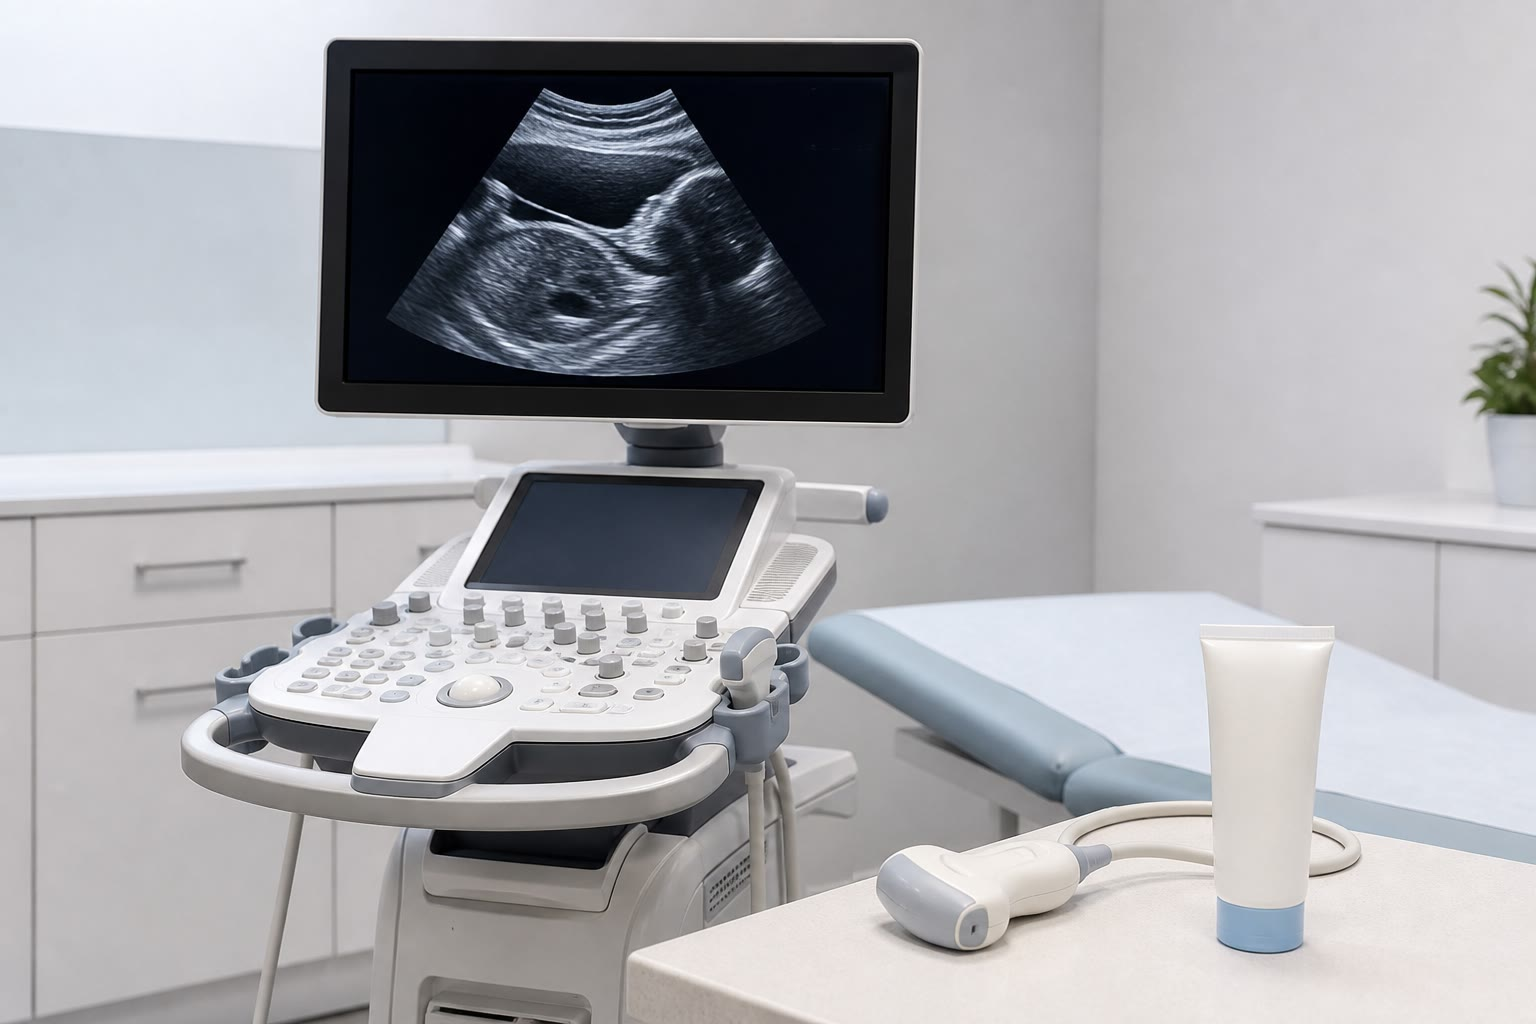
\includegraphics[width=0.58\linewidth]{images/book4/ai/b4-07-ultrasound-probe.jpg}

{\small Um aparelho de ultrassom: alguns megahertz de som, ecos cronometrados e os descasamentos de impedância entre tecidos desenham a imagem; o gel elimina a película de ar que refletiria tudo.}
\end{omfigure}

\section{Problema: Do trovão ao ecógrafo}

\begin{problem}[{Problema de fim de semana --- o som ao ar livre, numa sala
de concerto, dentro do corpo e vindo de uma sirene que passa}]
\label{pb:b2:sound-waves:1}

Ar: $\gamma = 1.40$, $M = \qty{29}{g/mol}$, $Z = \qty{410}{kg.m^{-2}.s^{-1}}$ a
\qty{15}{\degreeCelsius}; $R = \qty{8.31}{J/(mol.K)}$.

\medskip
\noindent\textbf{Parte I --- A tempestade.}
\begin{enumerate}
  \item \omterm{thm:b2:sound-waves:equation}{Velocidade do som} a \qty{15}{\degreeCelsius} e a \qty{30}{\degreeCelsius};
        justifique a regra dos "três segundos por quilômetro".
  \item O trovão chega \qty{4.0}{s} depois do clarão: distância da
        descarga. O trovão dura vários segundos, embora o clarão seja
        instantâneo: por quê?
  \item Perto da descarga o nível chega a \qty{120}{dB}: amplitude de pressão
        e amplitude de velocidade do ar.
  \item Energia recebida por metro quadrado de parede durante um trovão
        de \qty{2}{s} a \qty{120}{dB}.
  \item Numa noite clara o solo esfria e o ar fica mais frio embaixo
        do que em cima. Os raios sonoros obedecem à lei de Snell entre camadas,
        $\sin i/c = $ const.: os raios lançados para cima se curvam para baixo ou para cima?
        Por que os sons distantes são tão bem ouvidos à noite e sobre a água?
  \item De dia é o contrário: quem escuta a \qty{3}{km} não ouve nada.
        Estime o ângulo de que um raio horizontal se curvou depois de
        \qty{3}{km} se $c$ cai \qty{1}{\%} por \qty{500}{m} de altitude
        (trate a curvatura como uniforme: o raio é um círculo).

  \item O ar absorve as frequências altas muito mais que as baixas: por que
        o trovão distante ronca e o próximo estala?
\end{enumerate}

\medskip
\noindent\textbf{Parte II --- O concerto.}
Um alto-falante recebe \qty{100}{W} de potência elétrica e converte
$2\%$ dela em som, irradiado igualmente no semiespaço à sua
frente.
\begin{enumerate}[resume]
  \item Potência acústica; intensidade e nível a \qty{10}{m}.
  \item Amplitude de pressão ali; amplitudes de velocidade e de deslocamento
        a \qty{100}{Hz}.
  \item Nível a \qty{1}{m} (é seguro?) e distância em que a música
        cai a \qty{60}{dB}.
  \item Dez alto-falantes idênticos espalhados pelo palco, fora de
        fase: nível a \qty{10}{m}. Dois alto-falantes alimentados em fase, à
        mesma distância de um ouvinte no eixo deles: nível ali.
  \item A sala (volume \qty{10000}{m^3}) tem \qty{2000}{m^2} de paredes e plateia que absorvem $30\%$ do
        som que as atinge: estime a energia acústica armazenada na
        sala em equilíbrio e o tempo de reverberação (tempo para o
        nível cair \qty{60}{dB} depois que a música para), usando o
        balanço entre a potência emitida e a potência absorvida
        ($I_{\text{parede}} \approx ce/4$ para um campo difuso, admitido).
\end{enumerate}

\medskip
\noindent\textbf{Parte III --- O ecógrafo.}
Tecido mole: $c = \qty{1540}{m/s}$, $Z = \qty{1.6e6}{kg.m^{-2}.s^{-1}}$; osso,
$Z = \qty{7e6}{kg.m^{-2}.s^{-1}}$; ar, $\qty{400}{kg.m^{-2}.s^{-1}}$. Sob incidência
normal a amplitude de pressão refletida numa interface vale $r = (Z_2 -
Z_1)/(Z_2 + Z_1)$ vezes a incidente (deduzido em
\cref{ch:b2:wave-interfaces}); o tecido atenua o som cerca de
\qty{0.5}{dB} por centímetro e por megahertz.
\begin{enumerate}[resume]
  \item Comprimento de onda no tecido a \qty{3}{MHz}, \qty{5}{MHz} e \qty{10}{MHz}; o
        menor detalhe que cada um resolve é de cerca de um comprimento de onda.
  \item Atraso do eco de um órgão a \qty{12}{cm} de profundidade; taxa máxima com que
        os pulsos podem ser enviados sem confundir ecos; tempo para construir uma
        imagem de $200$ linhas.
  \item Fração da pressão, e da energia, refletida numa interface
        tecido--ar; numa interface tecido--osso; entre gordura
        ($Z = \qty{1.38e6}{kg.m^{-2}.s^{-1}}$) e músculo
        ($\qty{1.70e6}{kg.m^{-2}.s^{-1}}$). Por que o gel, e por que os ossos projetam
        sombras?
  \item A \qty{5}{MHz} o feixe atravessa \qty{2}{cm} de gordura antes de encontrar
        o músculo: fração da energia emitida que volta à
        sonda dessa interface (reflexão e atenuação de ida e
        volta), em \omterm{def:b2:sound-waves:decibel}{decibéis}.
  \item Atenuação de ida e volta em \omterm{def:b2:sound-waves:decibel}{decibéis} para o órgão da questão 12
        em cada uma das três frequências; se o aparelho suporta
        \qty{80}{dB} de perda, que frequências funcionam? Enuncie o compromisso
        entre resolução e profundidade.
  \item A sonda emite pulsos de \qty{1}{\micro s} a \qty{5}{MHz}: quantos
        comprimentos de onda tem um pulso, e como isso limita a resolução
        em profundidade?
  \item Modo Doppler a \qty{5}{MHz} numa artéria a \qty{0.40}{m/s}, feixe a
        \qty{60}{\degree}: desvio; o que o operador ouve.
\end{enumerate}

\medskip
\noindent\textbf{Parte IV --- A sirene.}
\begin{enumerate}[resume]
  \item Uma ambulância passa a \qty{90}{km/h} com uma sirene de \qty{700}{Hz}:
        frequências ouvidas na aproximação e no afastamento; o intervalo
        entre elas em semitons (um semitom é uma razão $2^{1/12}$).
  \item O ouvinte está num carro que anda a \qty{15}{m/s} rumo à
        ambulância que se aproxima: frequência ouvida.
  \item Em que instante alguém na calçada ouve exatamente
        \qty{700}{Hz}?
  \item As frentes de onda da ambulância à frente dela: comprimento de onda; celeridade
        do som em relação à ambulância, à frente e atrás.
  \item Um radar de \qty{24}{GHz} lê um desvio de \qty{3.2}{kHz} de um carro:
        celeridade do carro (a onda é deslocada duas vezes).
  \item Faça o balanço: as seis celeridades deste problema (som no ar, no
        tecido, a ambulância, o carro, as hemácias, a luz) e a
        única fórmula que dá conta de todas.
\end{enumerate}
\end{problem}
